\documentclass[a4paper]{article}
\usepackage{polski}
\usepackage[utf8]{inputenc}
\usepackage[pdftex]{hyperref}
\usepackage{makeidx}
\newtheorem{theorem}{Opis Filmu}
\usepackage[tableposition=top]{caption}
\usepackage{algorithmic}
\usepackage{graphicx}
\usepackage{enumerate}
\usepackage[T1]{fontenc}
\usepackage{hyperref}
\usepackage{multirow}
\usepackage{amsmath}
\usepackage{amssymb}
\author{Hubert Kozacz}
\title{Aniołowie Piekieł}
\begin{document}
\begin{abstract}
Artykuł na temat filmu "Aniołowie piekieł"
\end{abstract}
\tableofcontents
\section{Aniołowie Piekieł}
\begin{figure}[h!]
  \caption{Plakat Filmu}
  \centering
    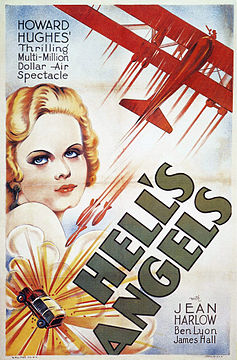
\includegraphics[width=0.5\textwidth]{pics/Poster.jpg}
\end{figure}

\begin{theorem}
\label{film}
\~{},,Aniołowie piekieł'' (ang. Hell’s Angels) – amerykański film z 1930, w reżyserii Edmunda Gouldinga, Howarda Hughesa oraz Jamesa Whale’a.
\end{theorem}

\section{Opis fabuły}
\begin{large}
\ref{film}
Tuż przed wybuchem I wojny światowej, bracia Monte i Roy Rutledge odwiedzają Niemcy wraz z ich niemieckim kolegą z Uniwersytetu Oksfordzkiego, Karlem. Kiedy wojna się rozpoczyna Karl zostaje wezwany do Niemiec, i trafia na pokład sterowca, który bombarduje później Londyn. Kieruje on bomby w taki sposób, że nieszkodliwie spadają do wody. Monte i Roy natomiast wstępują do RAF --- u. Nie są oni zadowoleni z powodu wojny, ale mimo to zostają ochotnikami do odbycia niebezpiecznej misji bombardowania niemieckiego składu amunicji.
\section{Obsada}

\begin{itemize}
  \item Ben Lyon --- Monte Rutledge
  \item James Hall --- Roy Rutledge
  \item Jean Harlow --- Helen (jako Jean Harlowe)
	\item John Darrow --- Karl Arnstedt 
\end{itemize}
\section {Nagrody i nominacje}

\begin{tabular}{ccc}
  Nazwa nagrody & Wygrane & Nominacje \\
	\hline
  Oscar & 1930 bez rezultatu & 1930 Najlepsze zdjęcia Harry Perry oraz Tony Gaudio \\
	\hline

\end{tabular}

\section{Bibliografia}
\begin{itemize}
\item \href {http://www.filmweb.pl/film/aniolowie+piekla-1930-37650}{Aniołowie piekieł} w bazie Filmweb
\item \href {http://www.imdb.com/title/tt0020960/}{Aniołowie piekieł} w bazie Internet Movie Database (ang.) 

\end{document}
